\documentclass[12pt, twoside]{article}
\usepackage[letterpaper, margin=1in, headsep=0.5in]{geometry}
\usepackage[english]{babel}
\usepackage[utf8]{inputenc}
\usepackage{amsmath}
\usepackage{amsfonts}
\usepackage{amssymb}
\usepackage{tikz}
%\usetikzlibrary{quotes, angles}

\usepackage{graphicx}
\usepackage{enumitem}
\usepackage{multicol}

\usepackage{fancyhdr}
\pagestyle{fancy}
\fancyhf{}
\renewcommand{\headrulewidth}{0pt} % disable the underline of the header

\fancyhead[RE]{\thepage}
\fancyhead[RO]{\thepage \\ Name: \hspace{3cm}}
\fancyhead[L]{BECA / Dr. Huson / 10th Grade Geometry\\* 15 January 2019}

\begin{document}
\subsubsection*{Classwork: Similar triangles, dilation ratios}
 \begin{enumerate}

   \item Triangle $ABC$ is dilated with a factor of $\frac{5}{3}$ centered at $A$, yielding $\triangle ADE$, as shown. Given $AB=9$, $BC=12$, and $AC=15$. \\[0.25cm] Find $AD$, $AE$, and $DE$. \vspace{1cm}
   \begin{center}
       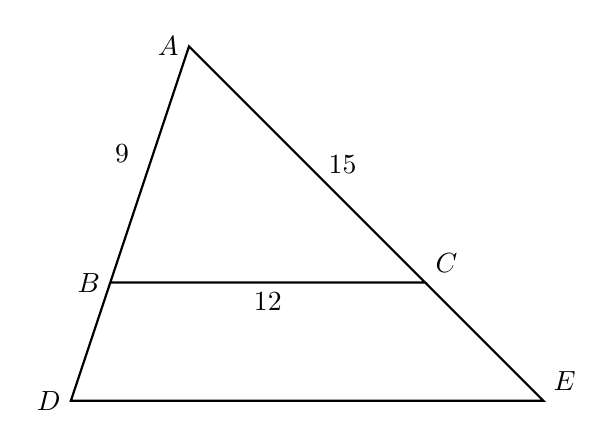
\begin{tikzpicture}[scale=0.5]
         \draw [thick]
         (0,0)node[left]{$B$}--
         (8,0)node[above right]{$C$}--
         (2,6)node[left]{$A$}--cycle;
         \draw [thick]
         (0,0)--
         (-1,-3)node[left]{$D$}--
         (11,-3)node[above right]{$E$}--(8,0);
         \node at (4,0)[below]{$12$};
         \node at (5.3, 3)[right]{$15$};
         \node at (0.3, 2.8)[above]{$9$};
       \end{tikzpicture}
     \end{center} \vspace{3cm}

   \item Given $\triangle ABP$ and $\triangle JKP$ as shown below. $\overline{AB} \parallel \overline{JK}$. $AP=5.7$, $JP=11.4$, and $JK=14.8$. Find $AB$.\\[0.5cm]
     \begin{tikzpicture}[scale=1.4]
         \draw [thick]
           (0.25,-1)node[right]{$B$}--
           (-0.5,2)node[left]{$K$}--
           (4,0)node[right]{$J$}--
           (0,0)node[above right]{$P$}--
           (-2,0)node[left]{$A$}--cycle;
       \end{tikzpicture}


  \newpage
  \item Regents problem:\\
  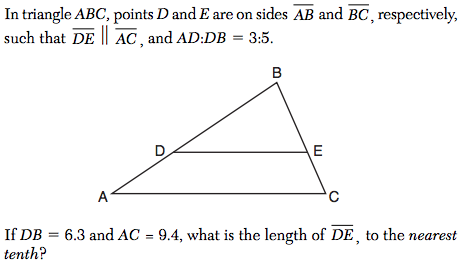
\includegraphics[width=0.7\textwidth]{similarity-ratio-spicy.png}\\[0.5cm]
  \vspace{2cm}

  \item Triangle $ADE$ and its midline $\overline{BC}$ are drawn, with $B$ the midpoint of $\overline{AD}$ and $C$ the midpoint of $\overline{AE}$. The two medians $\overline{AE}$ and $\overline{AE}$ are drawn, as shown, intersecting in point $F$, the centroid.\\[0.25cm]
  $\triangle FCB \sim \triangle FDE$ with scale factor $k=2$.\\[0.25cm]
  Given $BC=7$, find $DE$. \\[0.25cm] Given $BF=4$, find $FE$. \vspace{1cm}
  \begin{center}
      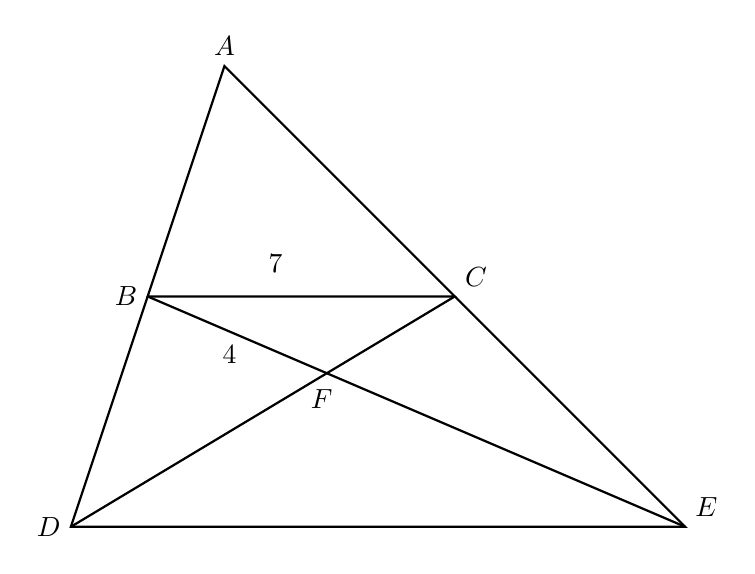
\begin{tikzpicture}[scale=0.65]
        \draw [thick]
        (0.5,1.5)node[left]{$B$}--
        (6.5,1.5)node[above right]{$C$}--
        (2,6)node[above]{$A$}--cycle;
        \draw [thick]
        (0.5,1.5)--
        (-1,-3)node[left]{$D$}--
        (11,-3)node[above right]{$E$}--(6.5,1.5);
        \draw [thick] (0.5,1.5)--(11,-3);
        \draw [thick] (6.5,1.5)--(-1,-3);
        \node at (3,2.5)[below]{$7$};
        \node at (3.5, -0.5)[right]{$F$};
        \node at (2.1, 0)[above]{$4$};
        %\node at (-0.7, -1)[above]{$5$};
      \end{tikzpicture}
    \end{center}



\end{enumerate}
\end{document}
